\chapter{Literature Review}
This literature review surveys fabric waste at the point of garment manufacturing, examines traditional pattern making processes, the advent and principles of zero waste design, the methods and rationale behind bespoke clothing, the concept of garment utility, and the impact of digitisation trends on these processes. By analysing these aspects, the review seeks to provide a comprehensive understanding of the current challenges and innovations in reducing fabric waste and how solutions that promote sustainable practice in the fashion industry can be formed. 

Example citation \cite{aldrich_metric_2015}

\section{Fabric Waste During Garment Manufacturing}
Fabric aste occurs at various stages of the manufacturing process, including cutting, sewing, and finishing. The cutting stage is particularly problematic, as patterns are not always optimized for fabric efficiency. The rigidity of traditional pattern making limits creativity and innovation, making it difficult to adapt to new sustainable practices, particularly on industrial scales.

In the context of minimizing fabric waste or recouping fabric waste, designers should consider garment utility. Garment utility refers to the functionality, durability, and versatility of a garment, as well as its aesthetic features that are desirable to the user. Enhancing garment utility can also involve incorporating fabric cut loss reduction into the garment’s design in creative ways, simultaneously increasing the garment’s overall appeal and lifespan. This is a core principle of ‘slow fashion’, which advocates for mindful consumption and long-term use of clothing. By focusing on garment utility, designers can create more sustainable fashion products that meet the needs of consumers while minimising environmental impact.

\section{Traditional Pattern Making}
Traditional pattern making involves the creation of two-dimensional templates for cutting fabric pieces. This process, outlined in Figure X, includes several critical steps, each carried out by individuals with specific roles. First, a designer creates a fashion sketch. A patternmarker then interprets the sketch into pieces, drafting a basic pattern block from specifications and measurements. Once this is established, grading is used to scale the pattern to different sizes, adding or subtracting specific amounts at strategic points to maintain the proportions of the original design. A marker-maker subsequently creates a marker, a layout of pattern pieces on fabric. Finally, the fabric is cut, and the pieces given to a sewer to assemble the garment.
\begin{figure} [H]
    \centering
    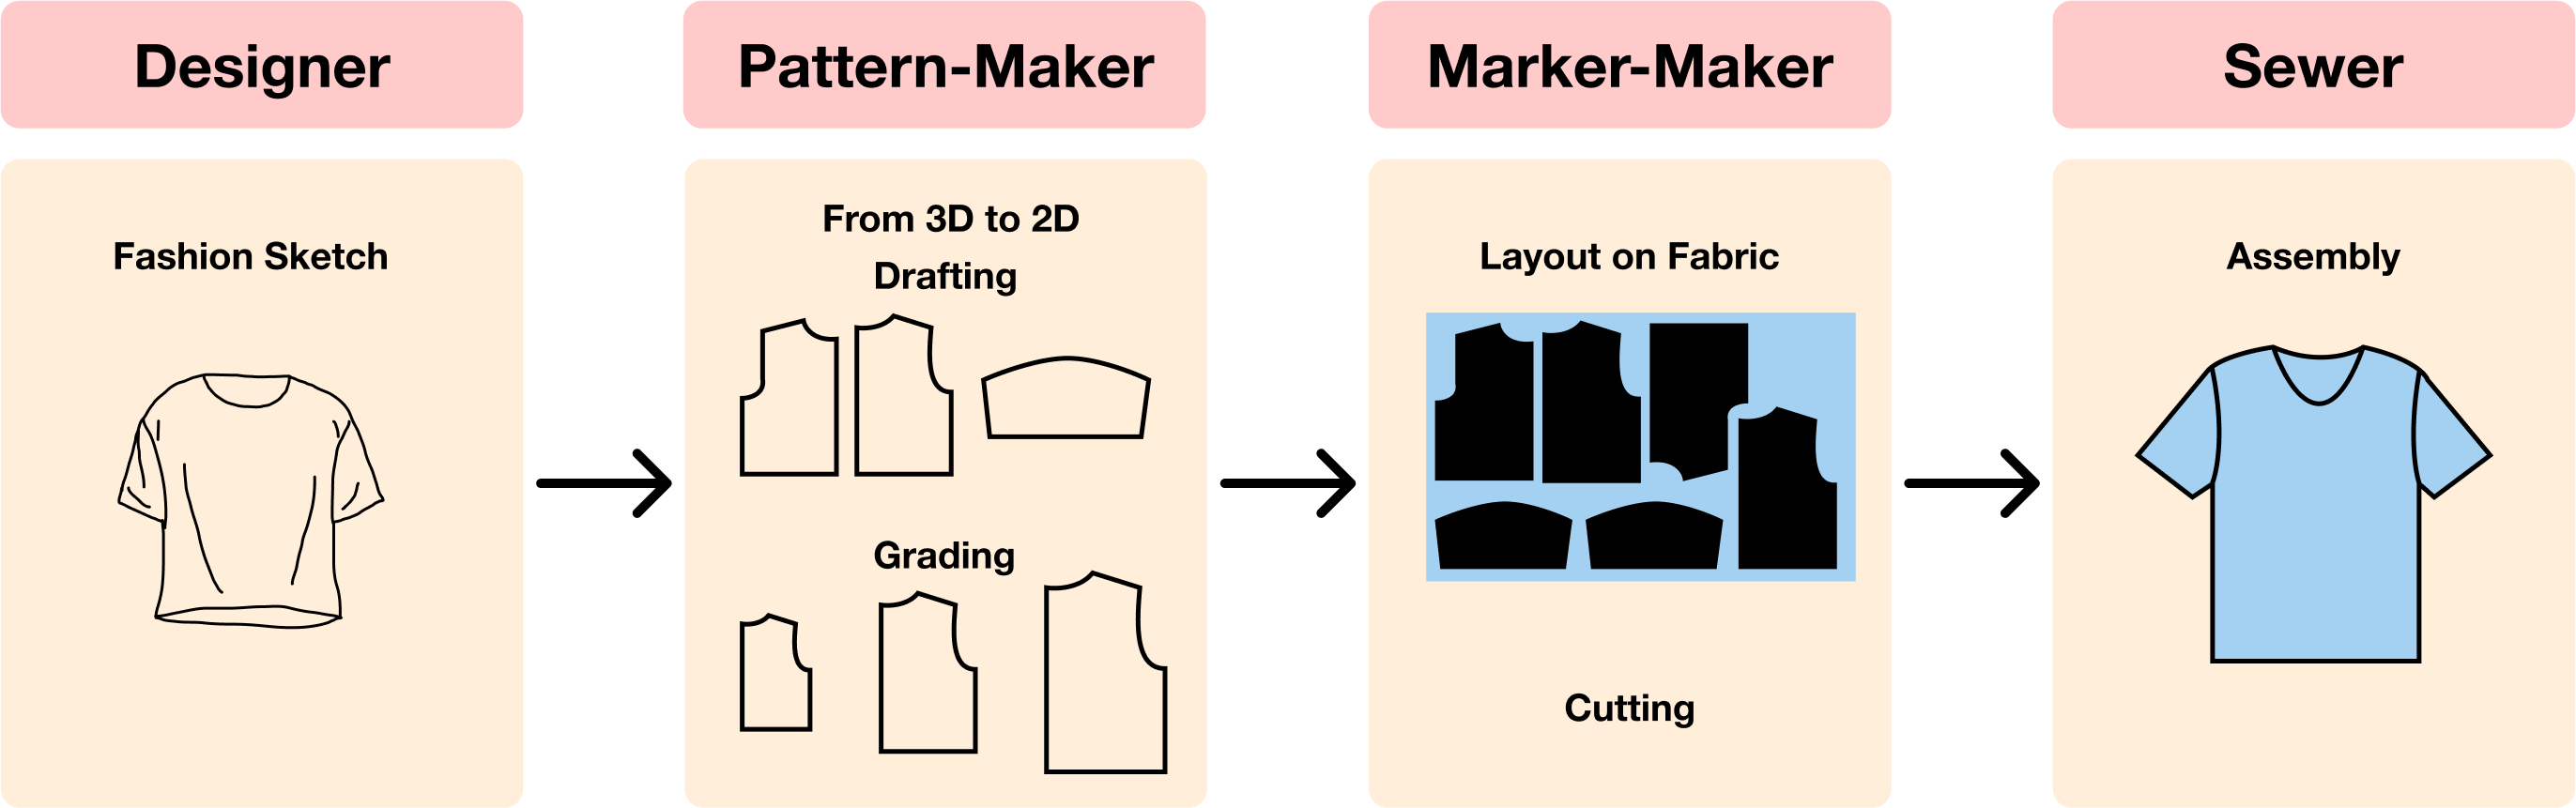
\includegraphics[width=0.8\textwidth]{Images/traditional process diagram.png}
    \caption{Traditional making flow}
\end{figure}
Grading has been criticised for its lack of inclusivity, as it often does not accommodate diverse body shapes and sizes. Examples abound of ‘big/tall’ sizes, ‘petite’ sizes, size nomenclature devoid of body measurements (e.g., ‘women’s size 6). Often, manufacturers do not make clothing in all sizes limiting consumer choice.

While effective for mass production, traditional methods often result in significant fabric waste. Traditional pattern pieces placed on a marker are cut out separately, surrounded by negative space. This separation often results in pieces not sharing borders, leading to unusable offcuts.  Even with advanced software and skilled manual marker-makers, fabric wastage remains north of 10\%. Fletcher critiques the fact that waste minimization is not integrated into the design phase, highlighting that the industry accepts these losses as an acceptable and inevitable part of the supply chain.
\begin{figure} [H]
    \centering
    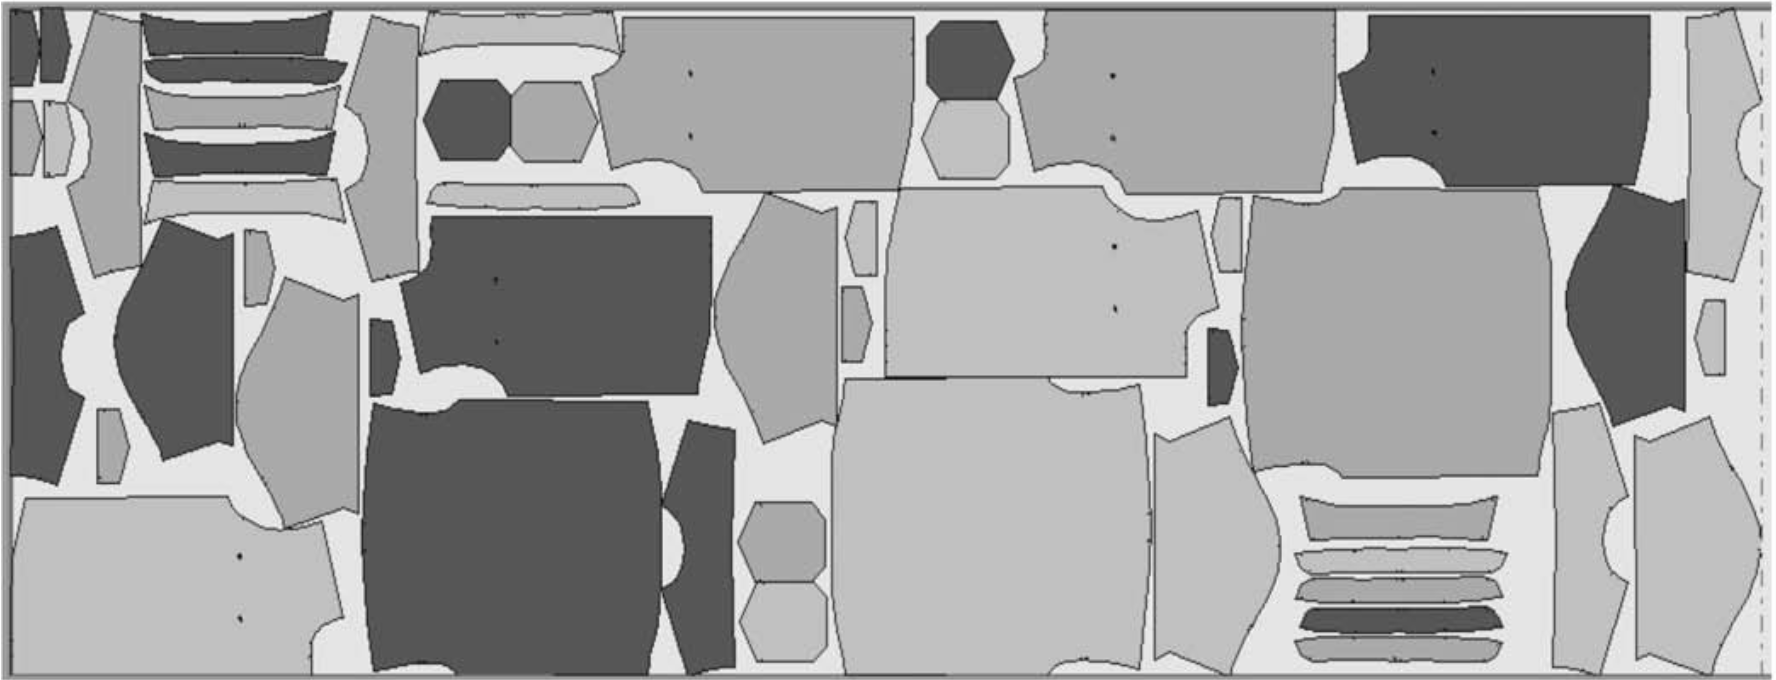
\includegraphics[width=\textwidth]{Images/digital marker layout.png}
    \caption{Digital marker layout example}
\end{figure}

\section{Zero Waste Pattern Making}
\subsection{Paradigm Shift}
Zero waste pattern design represents a paradigm shift in addressing fabric waste, constrasting sharply with traditional methods. This approach requires reimagining all conventional tailoring and textile techniques, with the fashion designer and patternmaker acting as one. Rissanen describes the aim is to "design a set of garment pieces that take up a given length of fabric in two dimensions...and the garment in three dimensions." Pattern making is pushed to its extremes as garment pieces are designed to fit together seamlessly, like a 'jigsaw puzzle,' to ensure no material is wasted. Incorporating fabric that would typically be wasted into the garment design is effectively enhances material utilization without increasing costs. Proponents in minimum-waste and zero-waste garment design deem passive participation in the existing system as insufficient and recognise this method demands continuous innovation and experimentation.

\subsection{Creative Imagination}
The effectiveness of zero waste cutting is highly dependent on the designer's creative imagination and problem-solving skills. There are no universal set of rules or formulas for creating zero waste patterns, as each design and context presents unique challenges. Moreover, because pattern pieces share borders, traditional pattern grading cannot be applied due to the complex relationships between pieces on the pattern. Imagination is crucial in navigating the constraints of fabric width and pattern interlocking to create functional and aesthetically pleasing garments. Key techniques involve utilising simple shapes, modularity, symmetry, and tessellation to fit the entire pattern into a compact rectangle. Depending on the fabric bolt, offcuts are either eliminated or come in rectangular shapes that are much easier to repurpose. Designers often use these offcuts in embellishments and mendings, adding new features structural integrity to the garment. The goal is to find the ideal bolt width given the pattern dimensions to reduce cut losses and to the increase cut loss utility through creative reuse.

\subsection{Application in Small Scale Domains}
Independent fashion designers and domestic sewers are currently leading the way in adopting zero-waste techniques, as companies are not yet making zero-waste garments for the mass market. While large-scale industry production often overlooks fabric efficiency, smaller-scale operations can experiment with and implement zero-waste designs more flexibly. This flexibility allows them to contribute to a reduction in fabric waste at a grassroots level. By integrating zero-waste principles, independent designers and home sewers can create unique, sustainable garments that challenge the norms of traditional fashion design and potentially transform their practices into successful businesses.

\subsection{Design Ease Aesthetic}
Because of simpler, modular shapes, zero waste garments are typically boxy and loose fitting with greater ease around the body. Ease is the difference between body measurements and garment measurements, and it significantly affects fit, comfort, and style. There are two types of ease: wearing ease and design ease. Wearing ease is the minimum amount of extra fabric needed to allow comfortable movement, while design ease involves additional fabric for aesthetic purposes. Zero waste pattern designs typically incorporate larger design ease to achieve their intended loose-fit aesthetic. This aesthetic is clearly seen in the aforementioned examples.

\subsection{Examples}
Here are some visuals to showcase aspects zero waste design process. Rissanen's Endurance Shirt II pattern in Figure X shows how he aims to fit pieces compactly into rectangular forms. Lei and Li proposes an innovative method to improve zero waste practice with their Segmentation and Reconstruction (SR) technique. SR breaks the fabric into multiple pieces that interlock to form the complete garment. This approach offers greater flexibility in design and fit adjustments, as the individual pattern pieces can be rearranged and modified more easily. As seen in Figure X, excess fabric is repurposed for functional embellishments like pockets and cuffs, which helps in minimizing waste and enhancing the garment’s utility. Figures X and X highlight the boxy and loose-fitting aesthetic of their designs.

\begin{figure} [H]
    \centering
    \rotatebox{270}{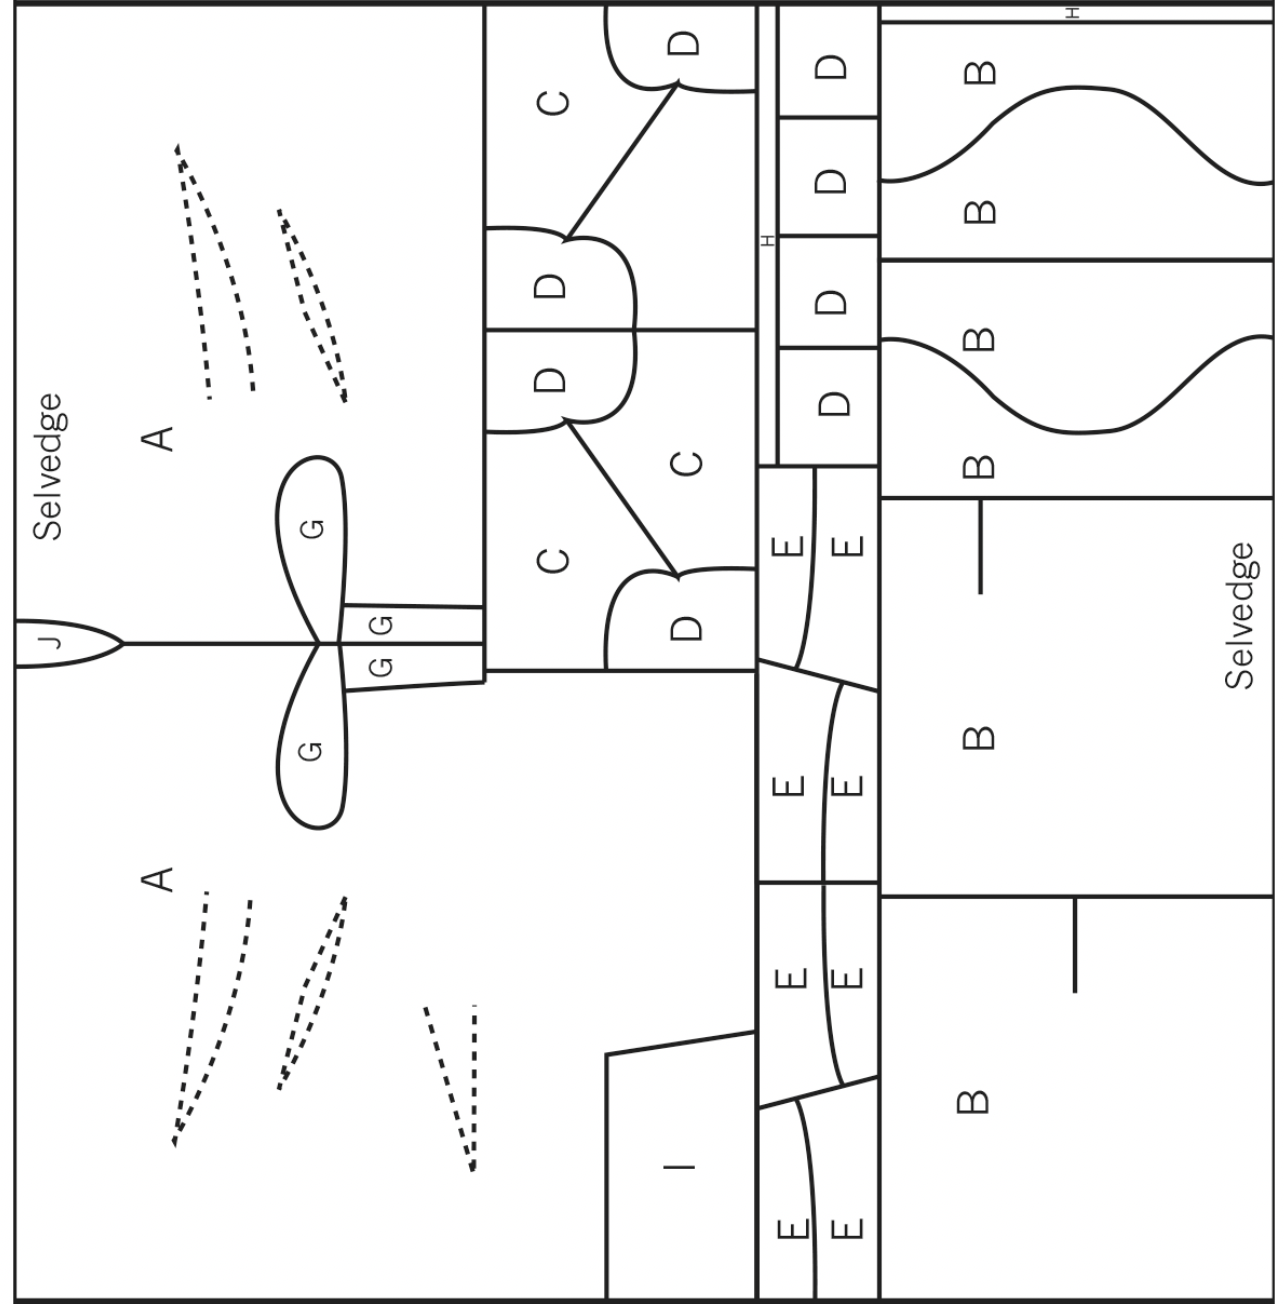
\includegraphics[width=0.8\textwidth]{Images/endurance shirt ii.png}}
    \caption{Endurance Shirt II block}
\end{figure}
\begin{figure} [H]
    \centering
    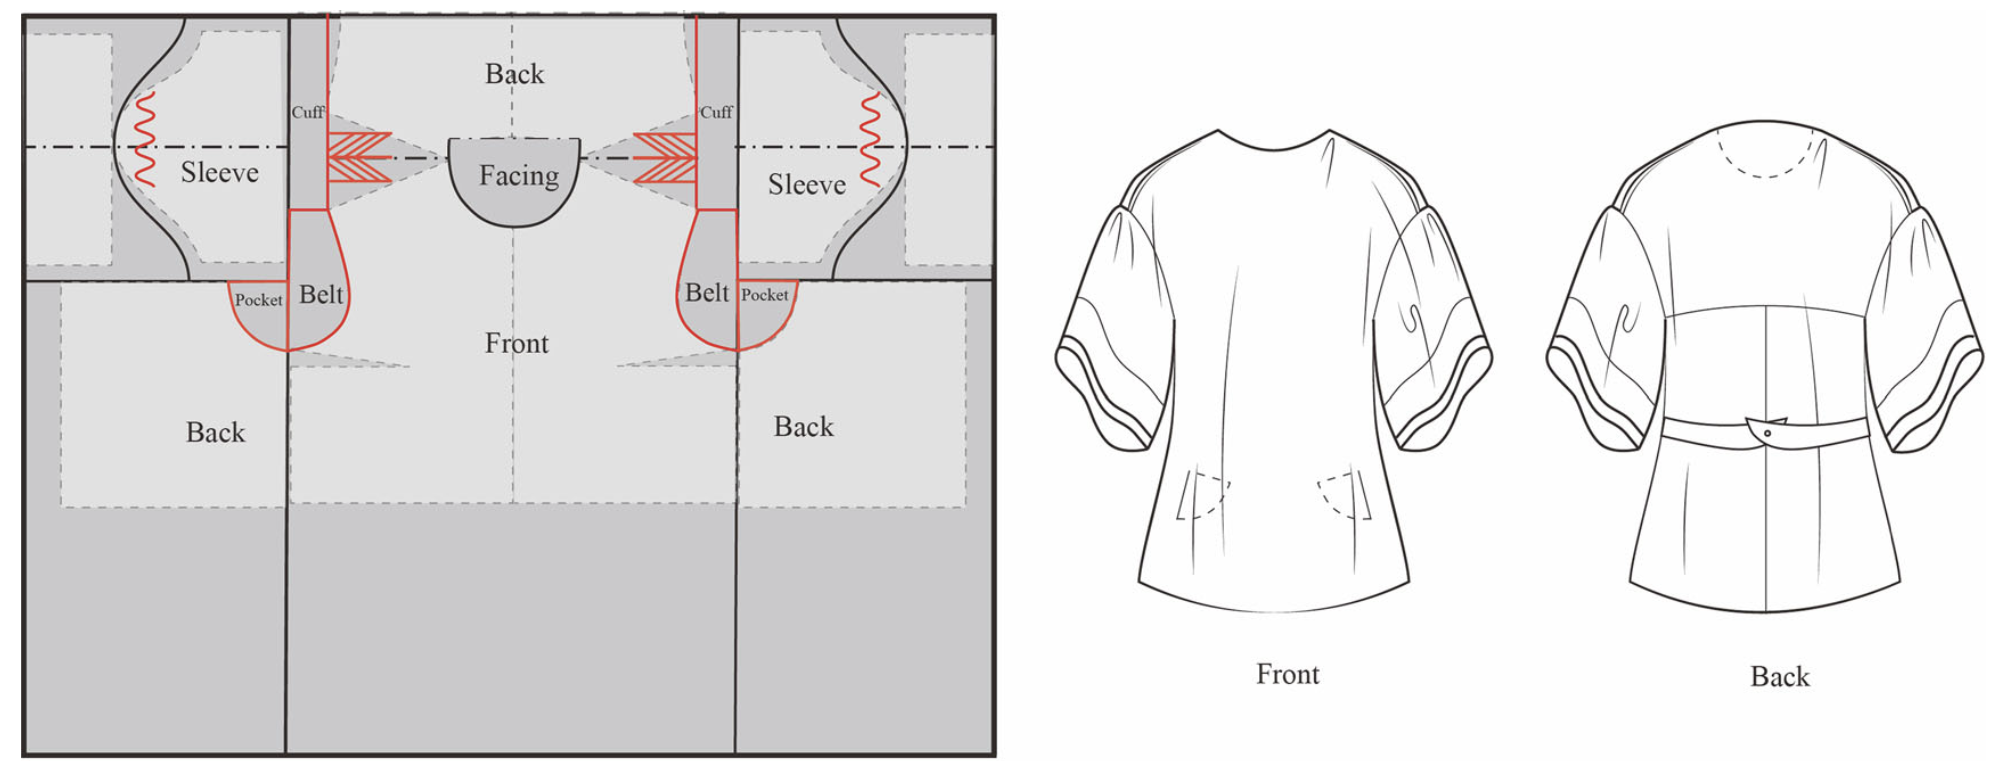
\includegraphics[width=\textwidth]{Images/SR kimono.png}
    \caption{SR kimono}
\end{figure}
\begin{figure} [H]
    \centering
    \begin{subfigure}[a]{0.6\textwidth}
        \centering
        
\includegraphics[width=\textwidth]{Images/rissanen jacket.png}
        \caption{Rissanen jacket}
    \end{subfigure}
    \hfill
    \begin{subfigure}[b]{0.3\textwidth}
        \centering
        
\includegraphics[width=\textwidth]{Images/bh tee.png}
        \caption{Helmersson zero waste tee}
    \end{subfigure}
    \caption{Examples showing boxy and loose fitting aesthetic}
\end{figure}

\section{Bespoke Clothing}
Fit and style are crucial factors for consumers when purchasing a garment. Achieving the right fit enhances satisfaction and extends the garment's life, reducing waste. Customization adjusts a garment to an individual's physical dimensions, while personalization reflects their unique style preferences. Together, they create bespoke clothing tailored to fit the individual's body and style, offering a sustainable alternative to mass-produced fashion.

Bespoke clothing also fosters a deeper connection between the garment and the wearer. Meticulous tailoring to personal measurements and style preferences increases the garment's significance, encouraging longer use and reducing the need for frequent replacements. This personalized approach contrasts with fast fashion's quick turnover and low cost, promoting more sustained use and lowering environmental impact.

The concept of a customized zero waste garment involves balancing fit and waste. Zero waste designs minimize fabric waste, while bespoke garments emphasize perfect fit and personalization. Exploring this tradeoff is crucial for developing sustainable, personalized fashion solutions that reconcile zero waste design with bespoke tailoring, contributing to more environmentally friendly and consumer-focused garment production.

\section{Digitisation Trends in Fashion}
Digitization is revolutionizing the fashion industry by transforming traditional methods of garment production and design with streamlined workflows. These technologies improve accuracy, efficiency, and sustainability, contributing to a more innovative and eco-friendly fashion industry.

\subsection{Body Scanning and Digital Pattern Making}
Body scanning technology provides precise measurements that enhance garment fit and customization. This technology utilizes 3D scanners to capture detailed body dimensions, resulting in accurate digital body models. Retailers such as Indochino and MTailor leverage body scanning to offer custom-fit garments, which enhances customer satisfaction and reduces fabric waste associated with ill-fitting clothes. Smartphones apps such as 3DLOOK provide a convenient way for consumers to scan their bodies at home, though not to the precision of professional scanning machines.

Digital pattern making complements body scanning by using the measurements to generate precise digital patterns tailored to individual dimensions. Software likes TUKAcad, and Optitex allows designers to create and adjust patterns efficiently. This digitization streamlines the pattern-making process, reducing errors and enhancing the production of bespoke clothing. These technologies collectively promote sustainable fashion practices by minimizing fabric waste and reducing the environmental impact of garment production.

\subsection{3D Modelling and Virtual Prototyping}
3D modeling and virtual prototyping enable designers to visualize and refine their creations before physical production. Software such as Marvelous Designer, Browzwear, and CLO 3D allows the creation of detailed digital representations of garments, complete with realistic textures and draping effects on avatars. Virtual prototyping offers several advantages, including reduced time and cost associated with producing physical samples, and the ability to experiment with different styles and materials virtually.

These technologies enhance collaboration within the fashion industry by allowing designers, pattern makers, and manufacturers to share and review digital prototypes, ensuring the final product meets design specifications. Virtual showrooms and fashion shows are also becoming more prevalent, offering brands a sustainable way to present collections globally without the environmental impact of physical events.

\subsection{Exisiting Computational Frameworks}
Computational frameworks in fashion design integrate various tools and software, enhancing innovation and efficiency. Platforms like GarmentCAD and FashionCAD automate the pattern-making and grading process, using algorithms to ensure accurate fit across different sizes, improving productivity and reduces errors as shown in the examples below.

\subsubsection{Apparel Design Engineering (ADE) Group}
Gill et al. from the University of Manchester's ADE Group explore the concept of parametric blocks in their study on evolving pattern practice. They highlight the transition from traditional patterns to bespoke parametric blocks, which offer significant advantages in terms of customizability and sustainability. Parametric pattern construction involves defining parameters based on measurements and preferences that establish the relationship between pattern inputs and outputs, enabling dynamic and geometrically associative patterns. This method supports the creation of custom garments.

\subsubsection{Generative Garment Design for Circularity (GGD4C)}
GGD4C proposes using generative algorithms to integrate lifecycle, material use, and circularity data at the garment design phase. This methodology shifts towards a more environmentally conscious fashion industry by incorporating circular design principles from the outset. The framework utilizes tools such as Grasshopper’s evolutionary solver Galapagos in Rhinoceros 3D software to create parametric patterns optimized for material efficiency and circularity. Early experiments with GGD4C, such as the design of a jumpsuit, have demonstrated its potential to reduce fabric waste and environmental impact significantly. The generative approach allows for the simultaneous optimization of multiple design objectives, aligning fashion design with sustainability goals.

\subsubsection{GarmentCode}
GarmentCode is a notable example of an advanced computational framework that applies object-oriented programming principles to garment construction. Its PyGarment library allows designers to create sewing patterns in a hierarchical, component-oriented manner. This approach enables the creation of complex, parametric garment designs that can be easily adjusted for different body measurements and styles. The system automates low-level tasks, such as placing darts, and supports the exploration of diverse design spaces. GarmentCode's configurator allows for the free manipulation of design parameters, enhancing creativity and efficiency in garment production.
\begin{figure} [H]
    \centering
    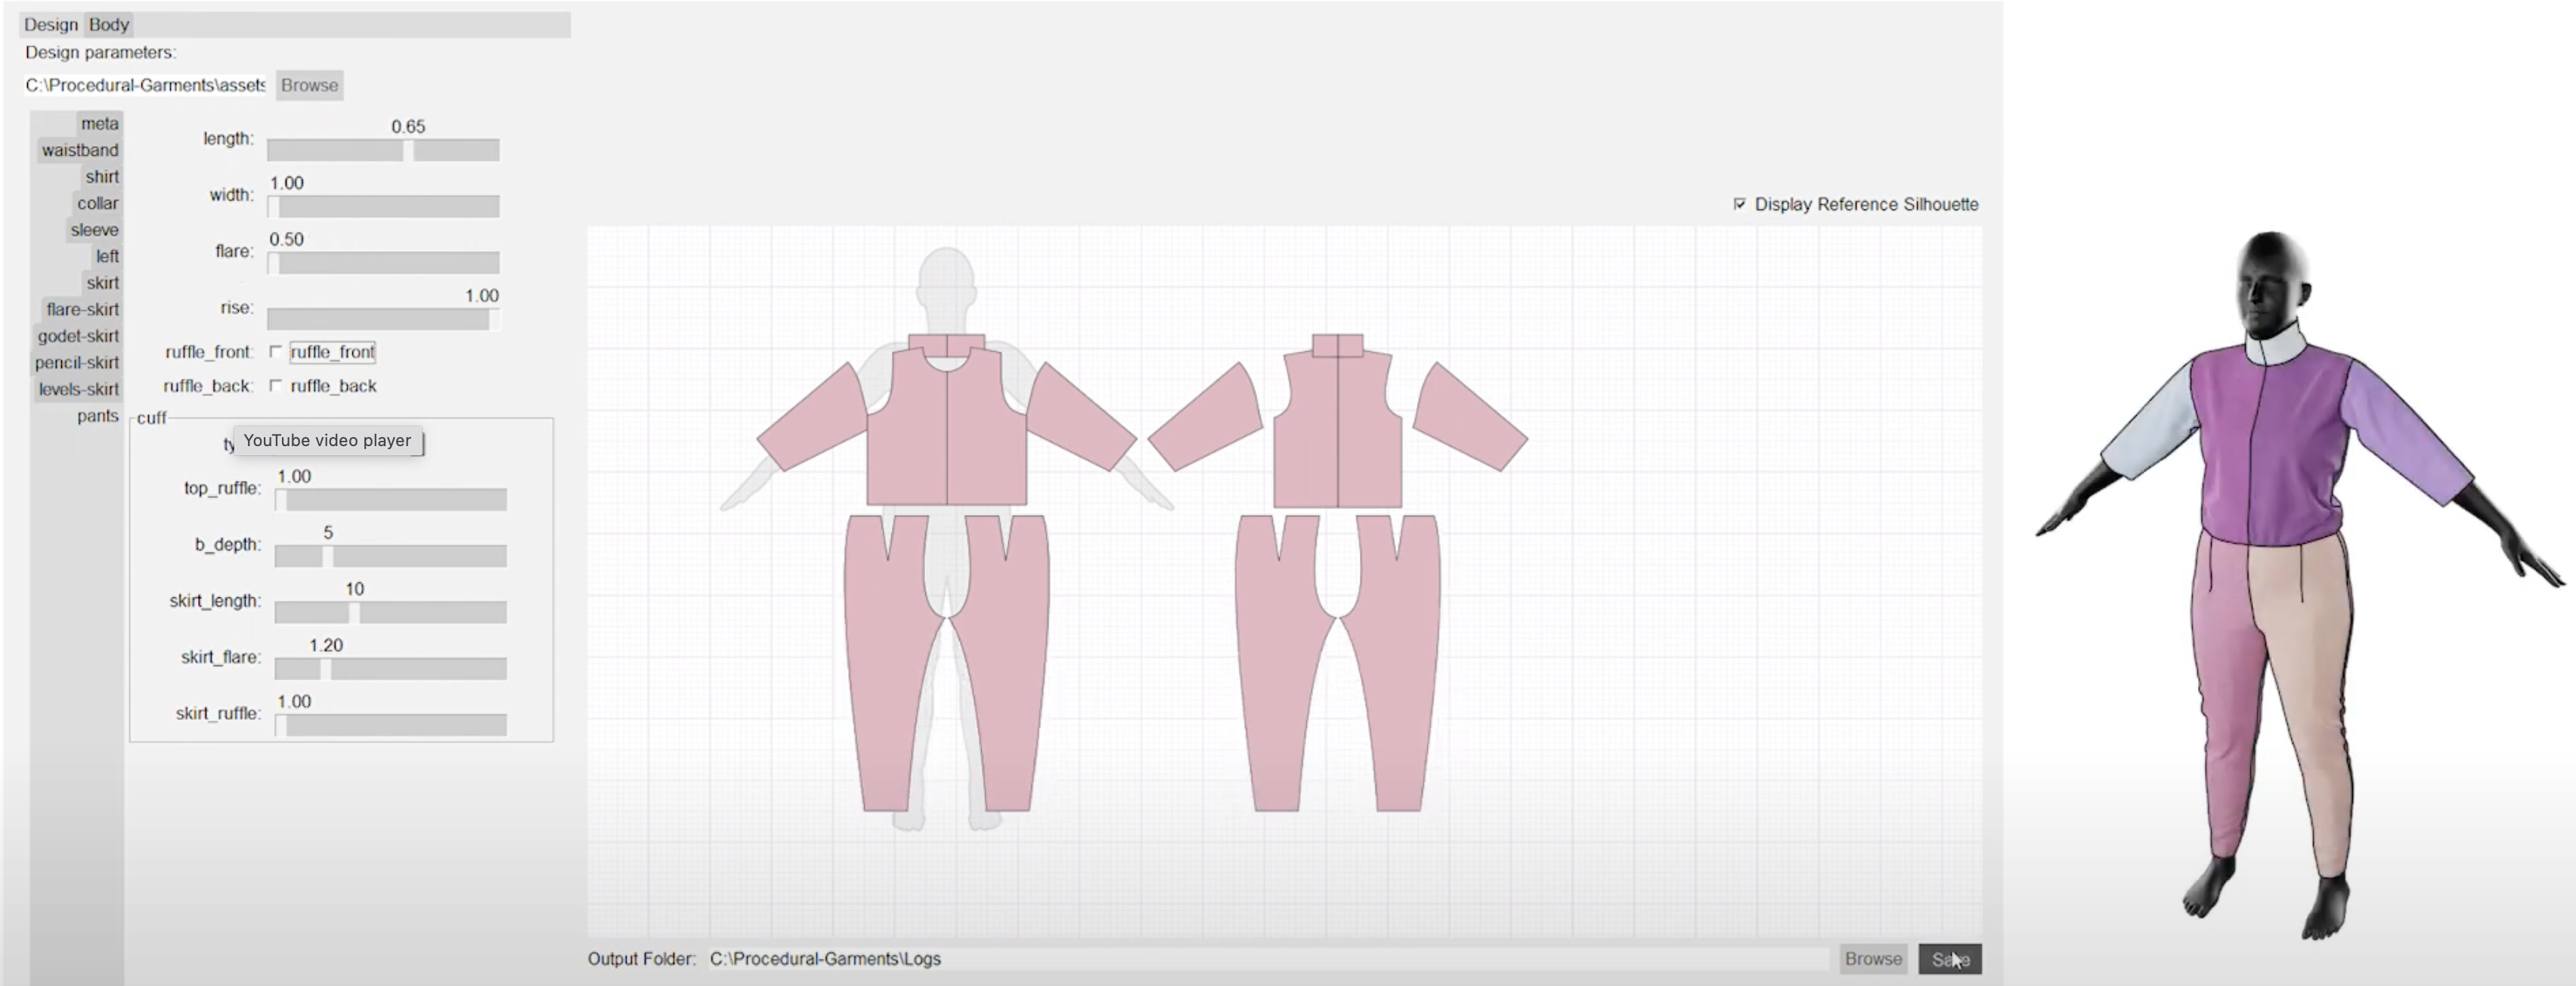
\includegraphics[width=0.8\textwidth]{Images/pygarment.png}
    \caption{Snapshot of GarmentCode GUI}
\end{figure}
